\documentclass[10pt]{article}
\usepackage{geometry}
\usepackage{graphicx}
\usepackage{wrapfig}
\usepackage{parskip}
\geometry{left=1.5cm,right=1.5cm,top=1.5cm,bottom=2cm}
\usepackage{gensymb}
\usepackage{caption}
\usepackage{xcolor}
\usepackage{amsmath}
\usepackage{float}  
\usepackage{subfigure}



\begin{document}


\title{\huge{COMP6245(20/21): Foundations of Machine Learning (MSc) Lab 2 Report}}
\author{\normalsize{Yan Zhang (yz10u20@soton.ac.uk)}}
\date{}
\maketitle

\section{Solution}
\subsection{Question 1}
In this report, I use perceptron algorithm to make prediction on the binary classification problem. For the training set $ D = \big\{x_i,y_i\big\} _{I=1}^{n}$ with features $x_i =  \begin{bmatrix}x_{i,1}&... &x_{i,d}  \end{bmatrix}^T \in  \Re ^d$, where $d$ is the number of features, and $n$ is the number of instances. And the outputs $y_i \in \Re$ is given from the set $\big\{0,1\big\}$

First, consider sample with n=100 comprising two data sets generated from two bi-variate Gaussian distributions with distinct means $m_1 = \begin{bmatrix}0 \\ 5\end{bmatrix}, m_2= \begin{bmatrix}5 \\ 0 \end{bmatrix}$, and identical covariance matrix $C = \begin{bmatrix} 2 & 1\\ 1 & 2\end{bmatrix}$. As the data is linear separable, the perceptron will find a separating hyperplane so that the data could be classified into two different types by updating the weights when it is classified incorrectly and integrates when all data are correctly classified.   

 Now, consider the problem with means $m_1 = \begin{bmatrix}2.5 \\ 2.5\end{bmatrix}, m_2= \begin{bmatrix}10 \\ 10 \end{bmatrix}$ and the covariance matrices equal. It is shown from the scatter plot that the data could not be separated by a line starting from the origin like before, with a low accuracy of training and testing. The solution to this is adding a bias to the threshold function, which is

\begin{equation}
    \centering
     f(x)  =\begin{cases}1 & if \ w \ast x + b >0, \\-1 & otherwise\end{cases} 
    \centering
\end{equation}

The value of $f(x)$ is used to classify a data point as either a positive or a negative instance, in the case of a binary classification problem. The bias b alters the position of decision boundary and shift the decision boundary away from the origin. As the training set is linearly separable, the perceptron will get to the state with all data classified correctly. 

The choice of learning rate also affects the performance of the classification, from the learning curve, it is clear that smaller alpha makes the algorithm learn more slowly and has a smaller fluctuation but sometimes will not reach the global minimal, larger alpha result in inefficient learning. There is a trade-off in the choice of learning rate, we could start from large alpha, and decrease the alpha value as in the process of learning

\begin{figure} %这里使用的是强制位置,除非真的放不下,不然就是写在哪里图就放在哪里,不会乱动
	\centering  %图片全局居中
	\vspace{-0.35cm} %设置与上面正文的距离
	\subfigtopskip=2pt %设置子图与上面正文或别的内容的距离
	\subfigbottomskip=2pt %设置第二行子图与第一行子图的距离,即下面的头与上面的脚的距离
	\subfigcapskip=-5pt %设置子图与子标题之间的距离
	\subfigure[The first data set]{
		\label{level.sub.1}
		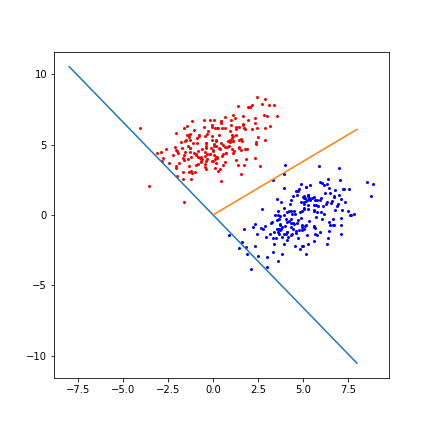
\includegraphics[width=0.32\linewidth]{decisionBoundary1.png}}
	\quad %默认情况下两个子图之间空的较少,使用这个命令加大宽度
	\subfigure[The second data set]{
		\label{level.sub.2}
		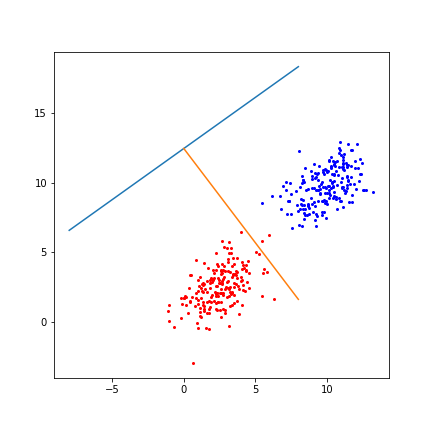
\includegraphics[width=0.32\linewidth]{decisionBoundary2.png}}
	  %这里是空了一行,能够实现强制将四张图分成两行两列显示,而不是放不下图了再换行,使用\\也行。
	\caption{Decision boundary(yellow line) in two different samples}
\end{figure}

\subsection{Question 2}

In order to test if the model could apply to other kind of data, I used the banknote authentication data set to make test using the Perceptron algorithm. The data is extracted from images that are taken from genuine and forged banknote-like specimens and transformed into continous variables. The data includes 4 attributes and 1 target variable, namely, variance of Wavelet Transformed image (continuous), skewness of Wavelet Transformed image (continuous), curtosis of Wavelet Transformed image (continuous), entropy of image (continuous) and class (integer:0, 1). 

In the case of banknote authentication data set, many attributes in different dimensions determine the outcome of the predicted target value. Thus, the parameter $w$ contains 5 random numbers, including a bias. Then, I set the learning rate $\alpha$ to be 0.1 and the maximal iteration time to be 5000. The Train and test set accuracy are both close to 1, the graph of learning curve of which is shown in Figure 2. 

Although, perceptron performs well on the data set, but there is only one neuron. If encountered with more complex problem with more attributes, perceptron may not generalize well. Thus, more neurons could be added in order to pursue better performance. Moreover, We could use a more advanced algorithm, like random forest, the prediction made from which is more accurate.

In conclusion, perceptron is a very simple and basic algorithm and it has many limitations. First, perceptron can only make correct prediction on the linearly separable cases. If the data are not linearly separable, the training process will never integrate. Second, the output of the model can only be one of the two values (0 or 1), which restricts generalization of algorithm. 



\begin{figure} %这里使用的是强制位置,除非真的放不下,不然就是写在哪里图就放在哪里,不会乱动
	\centering  %图片全局居中
	\vspace{-0.35cm} %设置与上面正文的距离
	\label{level.sub.1}
	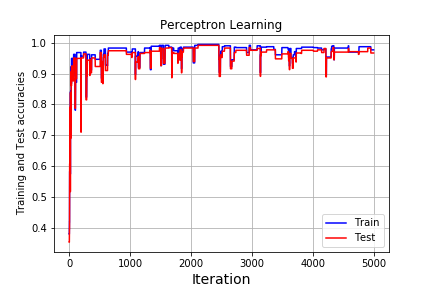
\includegraphics[width=0.32\linewidth]{LearningCurvesalpha0.002.png}
	\caption{The Perceptron learning curve of banknote authentication data}
\end{figure}

\end{document}


